% !TeX spellcheck = en_GB
% \section{ Comparison of Central Charged-Particle Densities}
\section{Comparison of Charged-Particle Densities at Central Rapidities}\label{chapter:discussion}
\label{sec:comparison_eta}
The~measured charged-particle densities in pseudorapidity near  $\eta\approx 0$ are compared to other experimental results from $pp$ and $p\bar{p}$ collisions (shown in Fig.~\ref{fig:comparison_eta}). Various event selections, based on the~topology of the~final state, allow to split the data samples into enhanced in non-\ac{SD} (NSD)  and  \ac{SD} events, whose  sum forms the~inelastic sample. For \ac{SD} events, 
the~midrapidity region  is  located at $\bar{\eta}=\eta_{m}=-\ln(\sqrt{s}/M_{X})$, instead of $\eta\approx 0$, and the~proper energy scale is given by $M_X$ instead of $\sqrt{s}$.
%In order to compare with \ac{ND} events, the SD and SD-enhanced results need to be calculated near $\bar{\eta}=\eta^\star=-\ln(\sqrt{s}/M_{X})$  at $\sqrt{s}=M_{X}$. 
The~values of $\eta_{m}$ and $\langle M_{X}\rangle$, calculated  for STAR data, are presented in Tab.~\ref{tab:etabarComparison}. 
For all three  ranges of $\xi$, the~value of $\eta_{m}$ is outside the~fiducial region of the measurement. In the~case of other experiments  the~pseudorapidity densities were obtained  in the~region of the~total number of primary charged particles $n_\textrm{ch}\geq1$  (instead of $n_\textrm{ch}\geq2$ as in these analyses).   Therefore, the~results from STAR  analysis were extrapolated  to the~above fiducial region using PYTHIA~8 A2 (MBR) \ac{SD}   predictions. The~uncertainties due to the~corrections are not estimated.

\begin{table}[h!]
	%\vspace{-0.3cm}
	\centering
	%\small
	\begin{tabular}{ |c|c|c|c| }
		\hline
		$\xi$ range &  $\langle M_X \rangle$ & $\eta_m$ & $\eta_\textrm{edge}$ \\
		\hline
		$0.02<\xi<0.05$ & $37.53$~GeV & $-1.67$ & $2.02$\\
		$0.05<\xi<0.1$ & $53.52$~GeV &  $-1.31$ & $2.73$\\
		$0.1<\xi<0.2$ & $72.71$~GeV & $-1.01$ & $3.34$\\
		\hline
	\end{tabular}
	\caption{Values of $\langle M_X \rangle$ and $\eta_m=\ln(\sqrt{s}/M_X)$ for three ranges of $\xi$ and position of gap edge $\eta_\textrm{edge}$.}
	\label{tab:etabarComparison}
	\vspace{0.8cm}
\end{table}

The~extrapolation procedure was as follows:
\begin{itemize} 
		\item the~ratio of particle density at $\bar{\eta}=\eta_{m}$ and $n_\textrm{ch}\geq1$ to that at $\bar{\eta}=0$ and $n_\textrm{ch}\geq2$ was calculated using PYTHIA~8 predictions,
		\item differences in the~slope of the~pseudorapidity distribution in the~region of $n_\textrm{ch}\geq2$ were observed between data and MC. Therefore, data and MC distributions were normalized to have the~same particle density at  $\bar{\eta}\approx 0$ and their ratio was fitted with
		a~linear function,
		
		 %in the~corresponding fiducial region of the~measurement,
		%\item the~ratios from step $\#1$  were multiplied by the~values of the~fitted functions at $\eta^\star$,
		\item  the~correction from step $\#1$,  multiplied by the~value of the~above function at $\bar{\eta}=\eta_{m}$, was used to scale the~measured particle density at $\bar{\eta}\approx0$. 
	
\end{itemize}
%The~measured and corrected charged-particle densities near $\bar{\eta}=\eta^\star$, $\rho_\textrm{M}$ and $\rho_\textrm{C}$, as well as the~corresponding scale factors, are shown in Tab.~\ref{tab:etabarComparison}.

\begin{comment}
Different procedure was used for events, in which the~value of $\eta^\star$ is outside the~fiducial region of the~measurement. 


A~single scale factor was obtained for events from the~ATLAS analysis, for which the~value of 
$\eta^\star$ is inside the~region of $|\eta|<2.5$. These scale factors are equal to $1$ for $\eta^\star=-1.47$ and $\eta^\star=-1.47$.
Different procedure was used for events in which  $\eta^\star$ is outside the~region of $|\eta|<0.7$ and $|\eta|<2.5$ for STAR and ATLAS analyses, respectively. The~ratios of the~measured charged-particle densities to those predicted by PYTHIA~8 were fitted with a~linear function in the~region of $|\eta|<0.7$ ($|\eta|<2.5$). This function was used to scale the~charged-particle densities obtained from PYTHIA~8 at $\eta^\star$. In both procedures, the~uncertainties due to the~corrections were not calculated.
\end{comment}




Figure~\ref{fig:comparison_eta} presents the~charged-particle densities near $\eta\approx 0$ as a~function of $\sqrt{s}$ in inelastic $pp$ and $p\bar{p}$ collisions. The~SD results, calculated near $\bar{\eta}=\eta_{m}$ at $\sqrt{s}$ $(M_X)$, are also shown.  
\begin{figure}[b!]
	%\centering
	\thisfloatpagestyle{fancy}
	%	\vspace*{-0.9\floatsep}
	\centering
	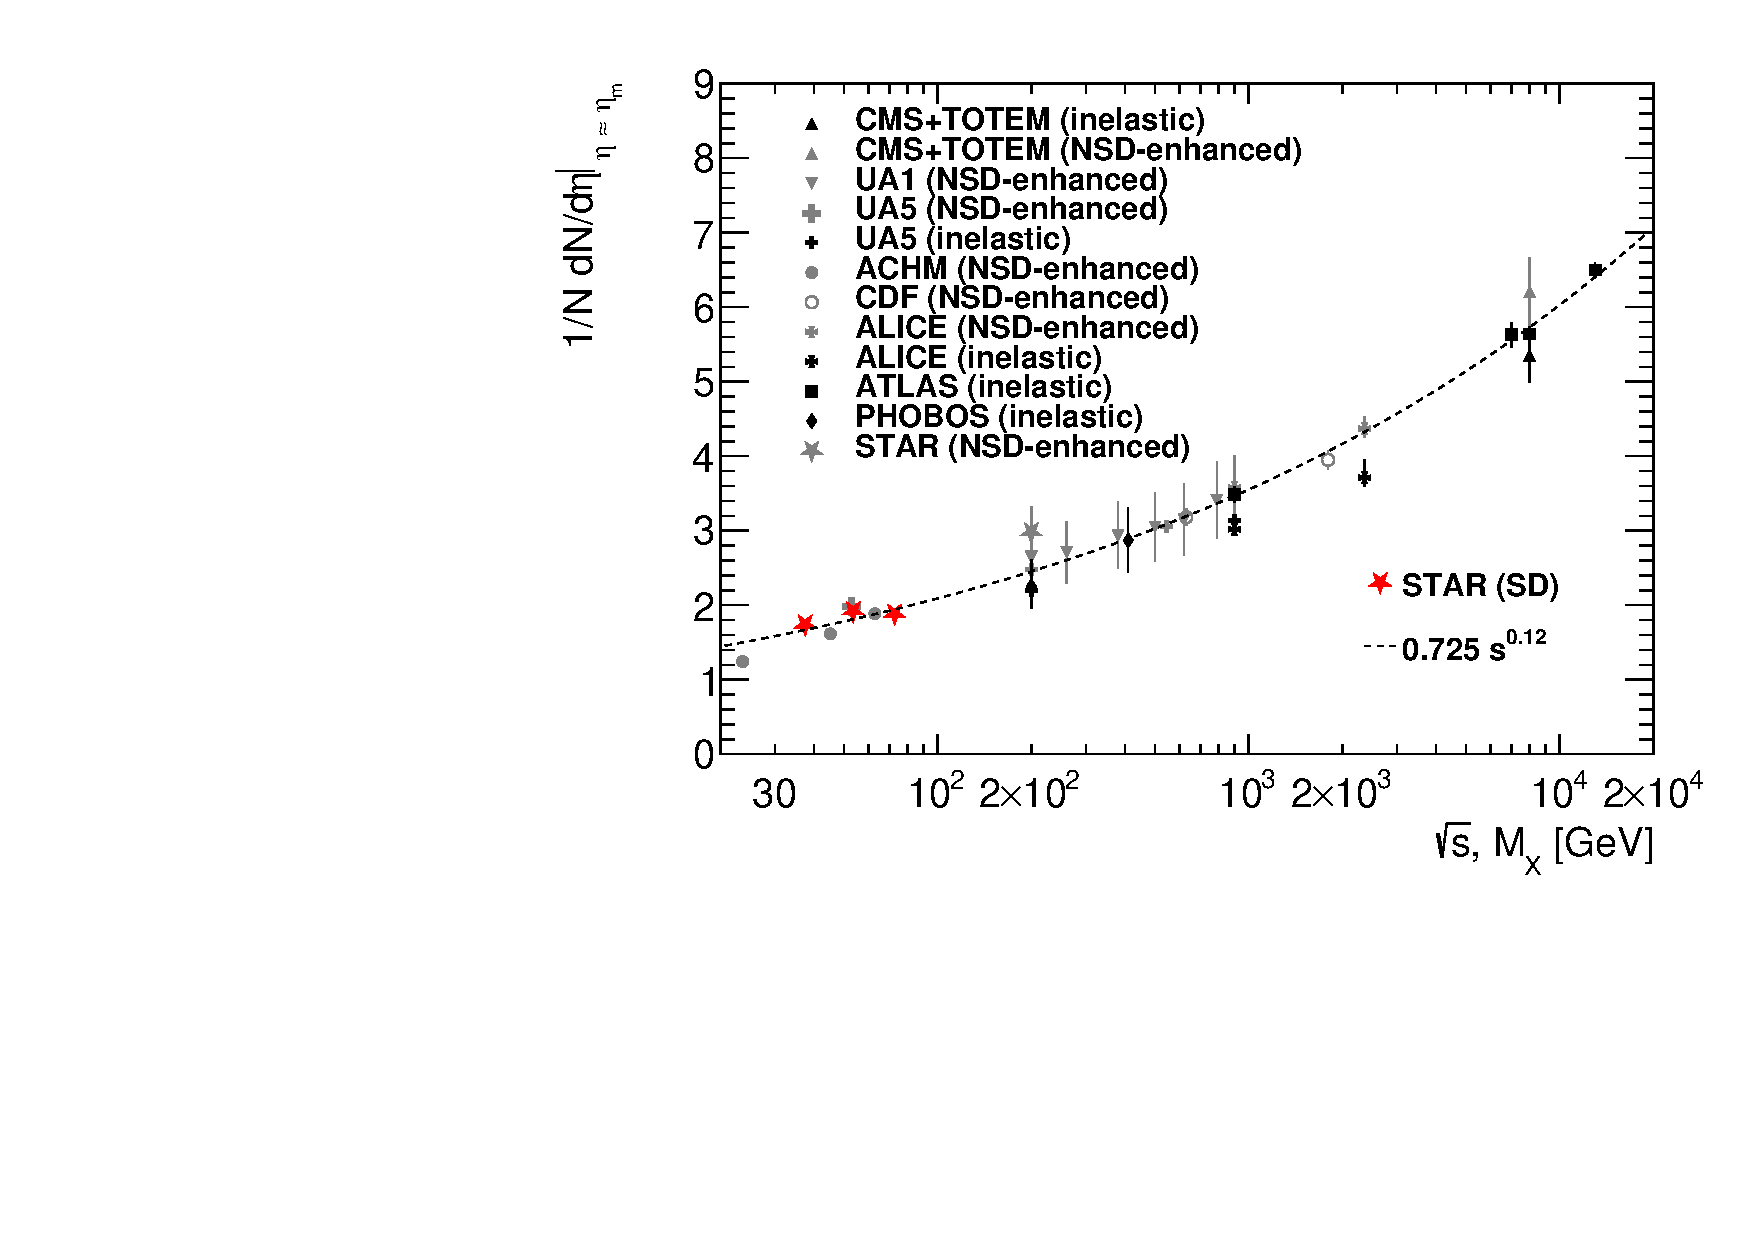
\includegraphics[width=1\textwidth,page=1]{chapters/discussion/img/dNdeta_sqrts.pdf}
	\vspace{-0.3cm}
	\caption{The evolution of $1/N_\textrm{ev}$ $dN/d\eta$ at $\eta\approx 0$ as a function of $\sqrt{s}$ in inelastic $pp$ and $p\bar{p}$ collisions~\cite{CMS:intro_3,UA1:intro_1,UA5:comparison,ISR:comparison,CDF:intro_2,ALICE:comparison,ATLAS:charged100,ATLAS:intro_2,ATLAS:intro_1,STAR:spectra,PHOBOS:intro}. The SD results were calculated near $\bar{\eta}\approx\eta_{m}$  at $\sqrt{s}$ $(M_X)$. The dashed lines represent power-law fits to the~NSD-enhanced~\cite{CMS:intro_3} data.
		The~results from this analysis are shown in red. }
	\label{fig:comparison_eta}
	%\vspace{-0.4cm}
\end{figure}

 



 

